
\chapter{Simulation}
The search for new physics at the LHC requires comprehensive modelling of the overwhelmingly large SM backgrounds. Particle physics events are simulated using Monte Carlo (MC) simulation that can be used, for example, to measure properties of known particles by comparison with data or to predict and optimize searches for BSM physics. Hence, simulation is generated for SM backgrounds using current theoretical knowledge, and BSM models are simulated using theoretical models.
There are four main stages; generation (GEN), simulation (SIM), digitisation (DIGI) and reconstruction (RECO). The GEN stage consists of producing the hard scattering between the partons from the protons and the outgoing particles. The SIM stage continues from the GEN stage simulating the paths of the outgoing particles through the detector after which the response of the detector is generated in the DIGI step. The RECO stage then uses the algorithms previously discussed in this chapter to produce collections of high-level physics objects which are the same as what is reconstructed in the detector from real data events.


\section{Monte Carlo Simulation Event Generators}

Event generators are used to simulate the signal and background processes at GEN-level. Using the proton PDFs and calculations of the Matrix Element (ME) associated to the Feynman diagrams for a particular process, a proton-proton collision can be replicated in simulation so that theory can be compared to experimental results. Due to the high-dimensional phase space associated to the multi-particle events produced at the LHC, Monte Carlo simulation is the only viable option. The \GEANTfour~\cite{GEANT4} program is used to perform the SIM-level simulation through the CMS detector. 

Figure~\ref{fig:MCGen}, shows the chain of processes which occur at GEN-level including:
\begin{itemize}
\item Incoming protons
\item Hard interaction of partons from inside proton
\item Parton shower from outgoing partons
\item Hadronisation of partons
\item Underlying event from the proton remnants 
\end{itemize}

\begin{figure}[ht!]
\begin{center}
    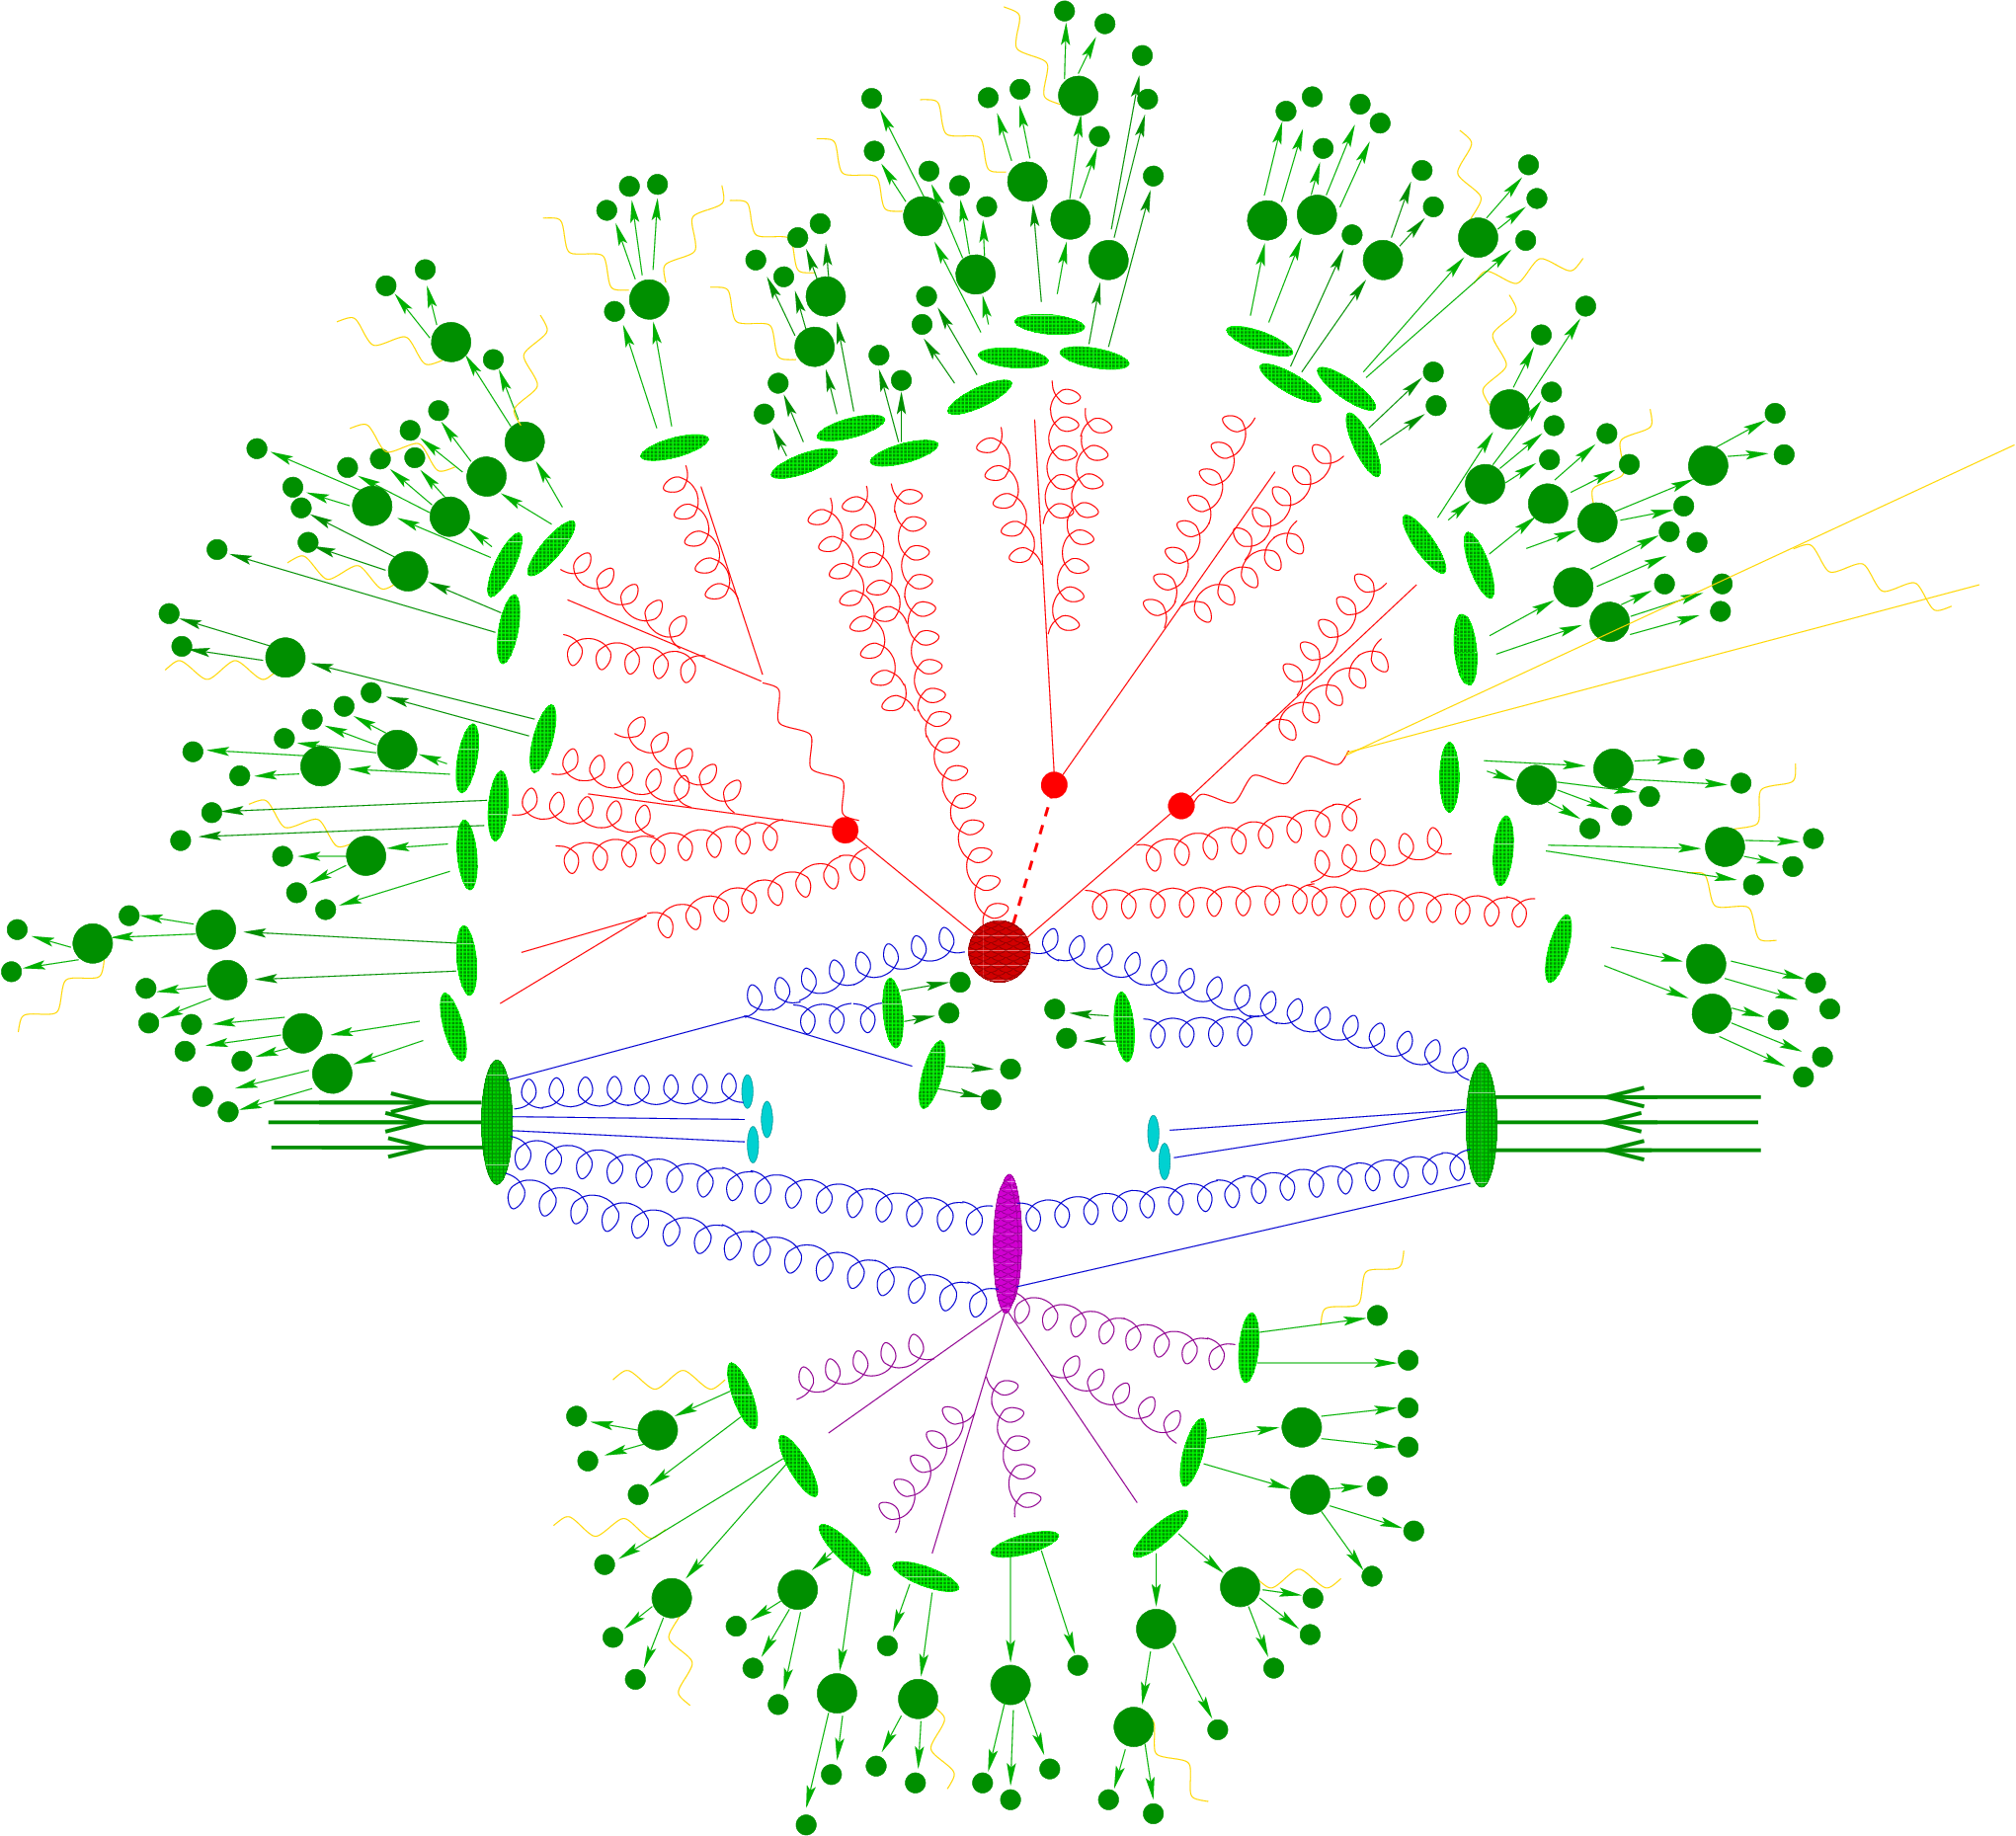
\includegraphics[width=0.7\textwidth]{images/eventGen.png}
    \caption{Depiction of hadron-hadron collision as simulated using an MC event generator. The red circle in the center indicates the hard collision. The surrounding tree-like structure represents Bremsstrahlung as simulated by parton showers. The purple circles represent a secondary hard scattering event. Light green ellipses represent parton to hadron transitions through hadronisation, darker green ellipses indicate hadron decays, and the yellow lines are soft photon radiation~\cite{Hoche:2014rga}.}
    \label{fig:MCGen}
\end{center}
\end{figure}

There are many MC event generators which specialise is one or more parts of the GEN-level simulation. Some generators are more specialised towards ME calculations and producing the hard interaction. Others are more optimised for simulating the parton shower, which is treated as a Markov process where four-momentum and probabilities are conserved with the creation of each new particle~\cite{Hoche:2014rga}.
Using generators above LO is a necessity when precision measurements are required and when many high-\pt and well-separated jets are present in the signature for the signal process~\cite{Degrande:2014sta}. The main event generators used in the thesis are as follows.

\subsection{\MADGRAPH}
\MADGRAPH is a leading-order (LO) event generator~\cite{Alwall2011} which calculates the ME at tree-level with a number of additional partons (which is process dependent and 	limited by computer memory contraints) for processes such as decays and $2\rightarrow n$ scattering. It takes PDF sets as input, for example NNPDF3.0 as shown in Fig.~\ref{fig:protonPDF}, which describes the kinematics of the incoming partons from the proton. It generates all Feynman diagrams for a particular process and evaluates each ME for a given phase space point. The number and type of partons and the kinematics of the event are generated.
\subsection{\aMCATNLO}
The \aMCATNLO package~\cite{Degrande:2014sta} can simulate events at next-to-leading order (NLO) in perturbative QCD as it uses both tree-level and one-loop perturbations. These additional corrections from higher-order Feynman diagrams make the simulation more accurate than its LO counterparts. This package includes initial and final state radiation. Initial state radiation (ISR) refers to any particle which is radiated off of an incoming particle to the collision whereas final state radiation (FSR) refers to a particle radiated off the final state outgoing products of a collision.\\
\subsubsection{Negative event weights}
By including higher order perturbations to the cross section calculated in \aMCATNLO, it is necessary to consider terms which interfere destructively. This is achieved by assigning negative weights to some events within the generator so that the differential cross section is simulated correctly. The effective number of events, $N_{eff}$, produced by the generator corresponds to $N^{pos} - N^{neg}$ (this equates to the number of events that would be produced for the given cross section) whereas the total number of events produced correspond to $N^{pos} + N^{neg}$. Therefore these samples can be scaled using the negative event weight, $W_{event}^{neg}$, according to Eq. (\ref{eqn:negativeScaling}).

\begin{equation}
\label{eqn:negativeScaling}
W_{event}^{neg} = \frac{N^{pos} + N^{neg}}{N^{pos} - N^{neg}} = \frac{N^{Total}}{ N^{Total} - 2\times N^{neg}}
\end{equation}


% \subsection{\POWHEG}
% The `Positive Weight Hardest Emission Generator', known as \POWHEG~\cite{POWHEG}, has the advantage that it is a NLO generator which only produces positive weight events due to the fact that it generates the hardest process in the event first. This means the double counting of the low-\pt radiation emitted, which happens in the \aMCATNLO generator, can be avoided.  
\subsection{\POWHEG}
The `Positive Weight Hardest Emission Generator', known as \POWHEG~\cite{POWHEG} generates the hardest process in the event first. This means that when it is interfaced with a shower MC (SMC) program for hadronisation which has emissions \pt-ordered, the double counting of the low-\pt radiation emitted can be avoided by using a \pt-veto. As the double counting of low-\pt emission is the cause for negative weight events, these can be avoided using \POWHEG with an SMC with \pt-ordering but negative weight events are still necessary for angular-ordered SMCs~\cite{Oleari:2010nx}. 


\subsection{\PYTHIA}
The \PYTHIA program~\cite{pythia} can take the parton-level event generated by another generator and add soft emissions from the initial and final state particles, as well as performing the fragmentation and hadronisation of quarks to produce the parton shower (PS). It can also simulate everything standalone including the initial protons fragmentation, multi-particle production, hadronisation, beam remnants and the underlying event. \PYTHIA is one of the most widely used generators amongst LHC experimentalists as it has been observed to produce particularly good agreement with data compared to other generators which produce parton showers.\\



\subsection{Matching}
``Matching'' or ``merging'' refers to the method of combining the output of the hard scatter, which has well separated particles, with parton showers which have much softer low-\pt particles. The \pt threshold at which partons from the ME are matched to the PS is known as the ME-PS threshold.
There are two types of matching used in \MADGRAPH depending on the order at which the process is generated~\cite{Degrande:2014sta}. At LO, MLM-merging is used to combine multiple LO$~+~$PS samples which are produced with different final-state multiplicities. FxFx-merging is similarly defined however NLO matrix elements are used.
